\documentclass[runningheads]{llncs}
\usepackage{graphicx}
\usepackage{float}
\usepackage{biblatex}
\usepackage{hyperref}

\addbibresource{references.bib}
\graphicspath{ {./images/} }

\begin{document}
\title{Data Mining}
\author{Eduardo Eloy}
\institute{Universidade de Évora, Portugal}
\maketitle             
\begin{abstract}
The Montesinho natural park in the northeast region of Portugal had several forest fires during the year of 2003.
And in this work I attempt to find a classification model that most accurately predicts the amount of area burned, the mean area burned in each fire, and the total number of fires for each pair of day of the week and month.
This was done by using 4 available regression functions in Weka to classify numerical attributes, Linear Reg, Gaussian Processes, SMO Reg and Multilayer Perceptron.
Although a bit limited due to the missing information on the pairs day of the week/month where no fires occurred this work could still be useful for improving resource management in firefighting.

\keywords{ regression,classification,sample,fire}
\end{abstract}

\section{Introduction}

In the interest of deepening out knowledge of data mining methods we were asked with choosing a dataset and identifying a problem (a prediction to make, a pattern to find etc) and solving it.

For that I chose the Forest Fires dataset from the "most popular" section of the Machine Leaning UCI Repository\cite{dataset}.
And with the 517 instances of forest fire data, which give information regarding the characteristic of each fire, I will build a model that predicts the mean area burned, number of fires and total area burned for each pair of day of the week (DOW) and month in the dataset (some pairs of DOW/Month had an insufficient number of instances)

This makes the problem significantly different from the relevant paper\cite{paper} in the UCI Repository page of this dataset.
The paper presents different approaches to different types of problems related to similar datasets, such as Vega-Garcia et al which adopted Neural Networks (NN)  to  predict human-caused wildfire occurrence and Stojanovaet al have appliyng Logistic Regression, Random Forest(RF) and Decision Trees(DT) to detect fire occurrence in Slovenian forests, using both satellite-based and meteorological data \cite{vega}.

The main approach in the paper uses non-costly meteorological data like rain,wind, temperature and  humidity and working the dataset through 5 different Data Mining techniques, these being multiple regression, Decision Trees, Random Forest, Neural Networks and a Support Vector Machine.
\break

\section{Data}
\subsubsection{Context}
\paragraph{}
The dataset relates to a national park in the northeast region of Portugal, Montesinho natural park\cite{montesinho} in 2003.
It is the result of an integration of 2 different datasets, it features, for each DOW/Month when there ocurred a forest fire, values relating to rain, wind, temperature and relative humidity (all measured by a meteorological station at the center of the park) at the affected x/y coordinates, the area burned (although registered as 0 if it was lower than 1 hectare) and 5 indices related to the Fire Weather Index\cite{fwi}
In total it has 517 instances each with 13 attributes.

As Portugal is a country with a damaging fire season in the summer months\cite{ptfire} it remains relevant to observe data of this type to assess the characteristics of fire prone locations and periods (day of the week and months).

The dataset has been used in the following publication \break
[Cortez and Morais, 2007] P. Cortez and A. Morais. A Data Mining Approach to Predict Forest Fires using Meteorological Data. In J. Neves, M. F. Santos and J. Machado Eds., New Trends in Artificial Intelligence, Proceedings of the 13th EPIA 2007 - Portuguese Conference on Artificial Intelligence, December, Guimarães, Portugal, pp. 512-523, 2007. APPIA, ISBN-13 978-989-95618-0-9.

\subsection{Attributes}
\paragraph{}

1. X - x-axis spatial coordinate within the Montesinho park map: 1 to 9\hfill\break{}
2. Y - y-axis spatial coordinate within the Montesinho park map: 2 to 9\hfill\break{}
3. month - month of the year: 'jan' to 'dec'\hfill\break{}
4. day - day of the week: 'mon' to 'sun'\hfill\break{}
5. FFMC - FFMC index from the FWI system: 18.7 to 96.20\hfill\break{}
6. DMC - DMC index from the FWI system: 1.1 to 291.3\hfill\break{}
7. DC - DC index from the FWI system: 7.9 to 860.6\hfill\break{}
8. ISI - ISI index from the FWI system: 0.0 to 56.10\hfill\break{}
9. temp - temperature in Celsius degrees: 2.2 to 33.30\hfill\break{}
10. RH - relative humidity in %: 15.0 to 100\hfill\break{}
11. wind - wind speed in km/h: 0.40 to 9.40\hfill\break{}
12. rain - outside rain in mm/m2 : 0.0 to 6.4\hfill\break{}
13. area - the burned area of the forest (in ha): 0.00 to 1090.84\hfill

\section{Algorithms}
\subsection{Justification}
The problem being one of regression, it ought to be verified whether it actually makes sense to apply this method to predict the 3 attributes.
This will be done by plotting histograms of the area burned and the number of fires (that burned that amount of area) during the whole year, and additionally, because the months of June, July, August and September are representative of the dataset, a sample with just these months will be analyzed. This sample has 405 instances, making up for 78.33\% of the dataset.
In every one of the following histograms the results are the same, the decrease in the number of fires per burned area is exponential, and it's clear that most of the fires are in the 0 (below 1 ha) and 1-50 range.
\
\begin{figure}
    \caption{Histogram of the whole year's fires}\label{hist1}
    \centerline{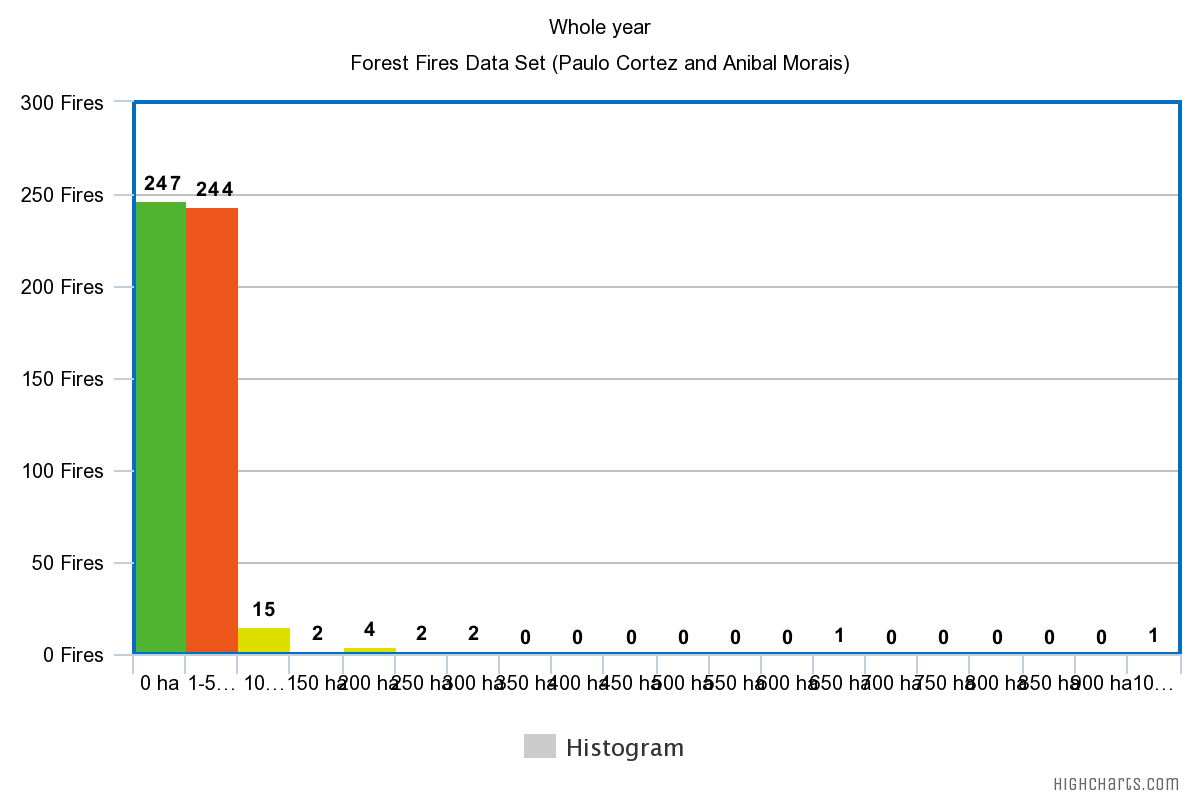
\includegraphics[width=1\columnwidth]{imagens/WholeYear.png}}
    \label{WholeY}
\end{figure} 
\begin{figure}
    \caption{Histogram of the whole year's fires with linear scale}\label{hist2}
    \centerline{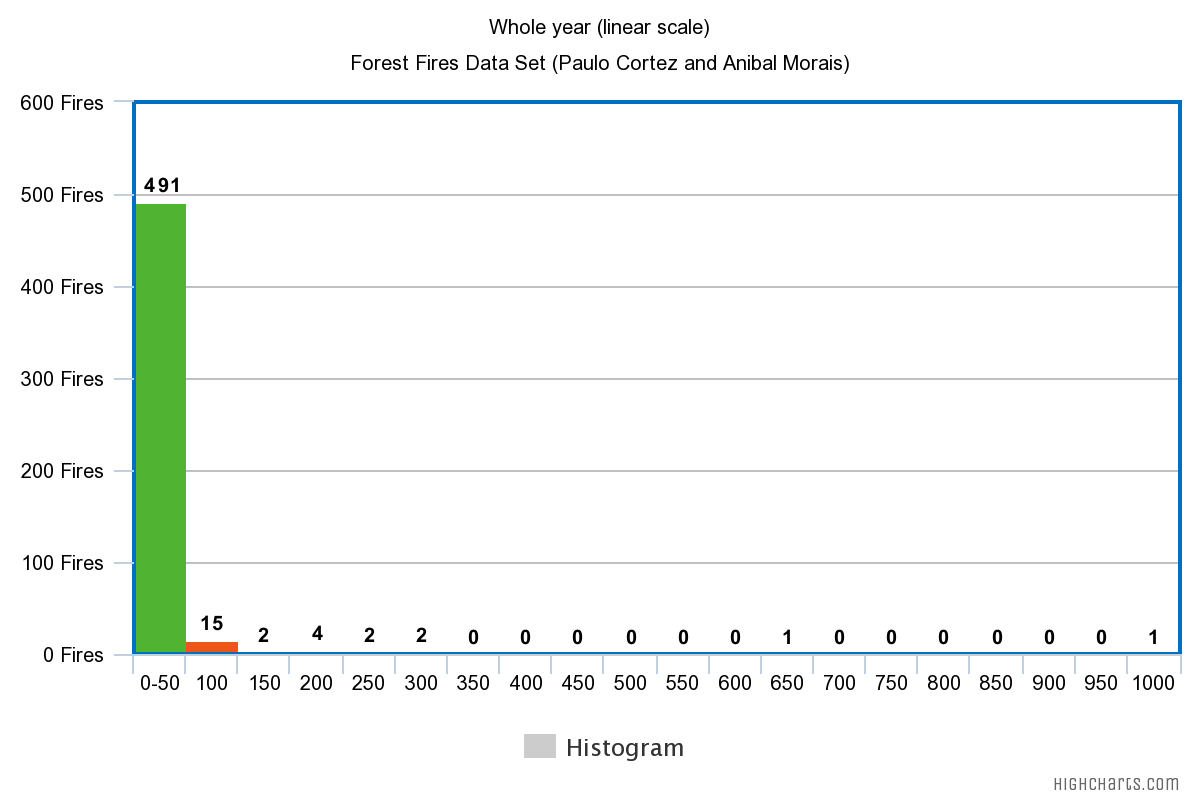
\includegraphics[width=1\columnwidth]{imagens/WholeYearLinear.png}}
    \label{WholeYL}
\end{figure}

\begin{figure}
    \caption{Histogram of the summer's fires}\label{hist3}
    \centerline{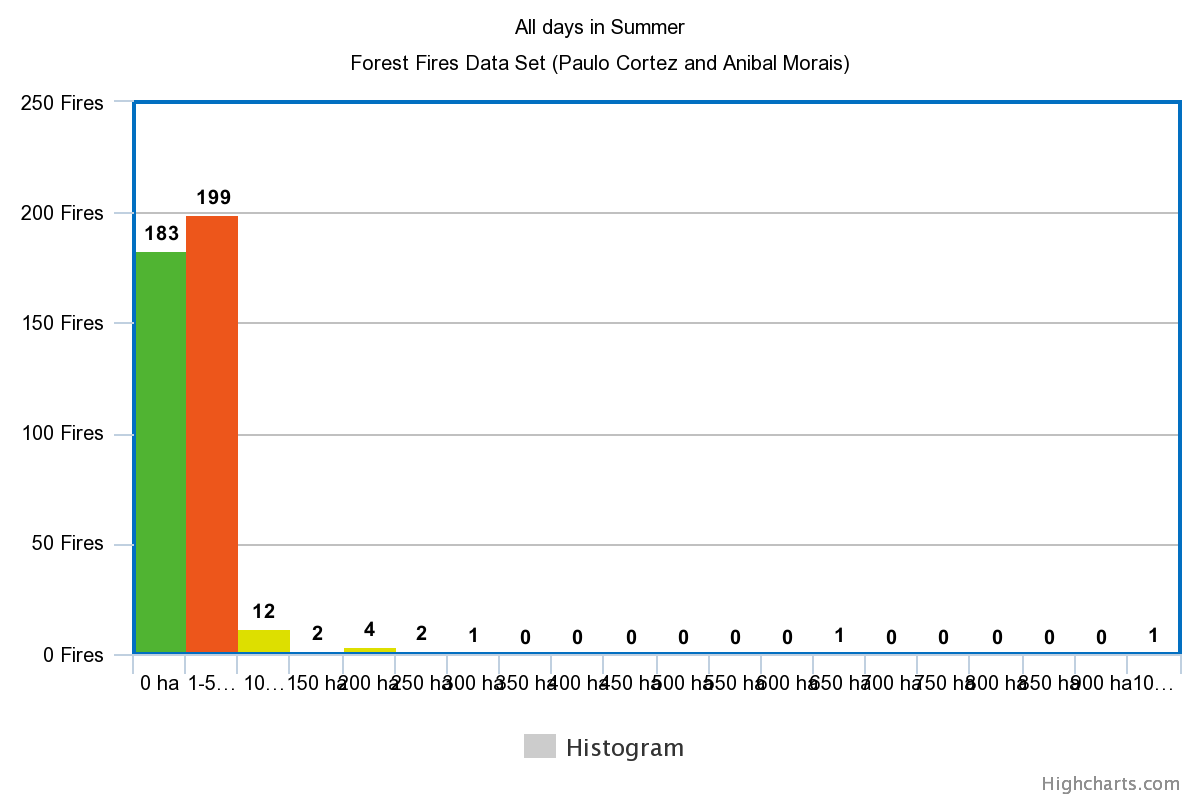
\includegraphics[width=1\columnwidth]{imagens/AllSummer.png}}
    \label{Summ}
\end{figure}
\begin{figure}
    \caption{Histogram of the summer's fires with linear scale}\label{hist4}
    \centerline{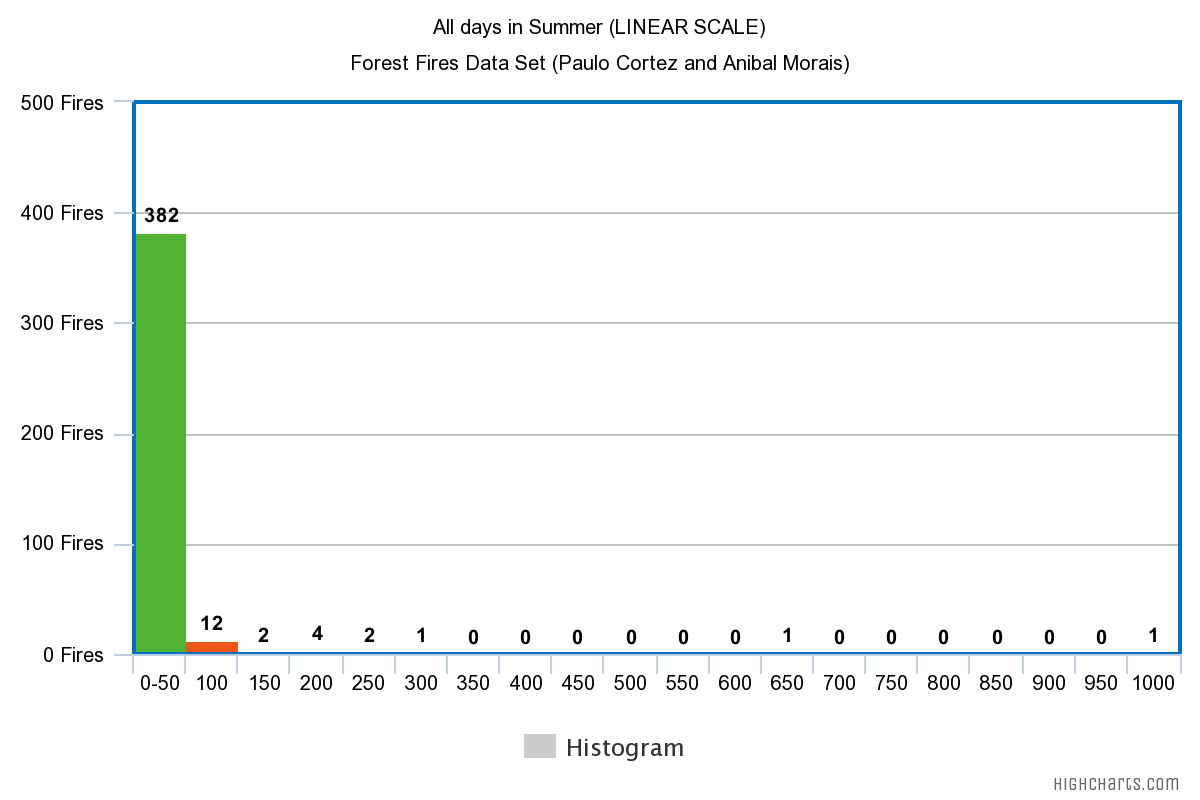
\includegraphics[width=1\columnwidth]{imagens/AllSummerLinear.png}}
    \label{SummL}
\end{figure}
\break
\subsection{Pre-Process}
\paragraph{}

The dataset will be modified, since the targets of the predictions are the mean areas, number of fires and total area burned for each DOW/Month. So the aggregation of the instances will be done by their DOW/Month. Meaning one instance in the aggregated dataset could be, for example, the characteristics of the Sundays in August.
The X and Y coordinates can't be aggregated since they are unique to each location so these 2.
attributes will be deleted, however, 3 new attributes will be added:
\hfill\break{}
numberOfFires - total number of fires in all DAYS of MONTH\hfill\break{}
totalAreaBurned - total area burned by fires in all DAYS of MONTH\hfill\break{}
meanArea - mean area burned in every fire for a given DAY of MONTH\hfill\break{}
The remaining attributes like temperature and other FWI indices will be added up and then divided by the number of instances giving us their average, for example, the average FMC of the Saturdays in January is 82.1.

After running an aggregation script with the whole dataset, the resulting dataset has 64 instances.
One might think that the aggregation would result in 7*12=84 instances, this isn't the case because some pairs of DAY/Month just don't have registered fires.
The aggregated summer sample results in 27 instances.

\subsection{Regression Algorithms}
\paragraph{}

In default Weka there are 4 available regression functions to this dataset:\break

Linear Regression\cite{lin}: The most simple of the 4 regression algorithms, Linear Regression builds linear models by using linear predictor functions that estimate their parameters from the data.\hfill\break{}
Sequential minimal optimization regression\cite{smo}: This algorithm trains a support vector machine by breaking down large Quadratic Programming problems into smaller Quadratic Programming problems and solving them.\hfill\break{}
Gaussian Process Regression\cite{gp}: Also known as Kriging, is an interpolation method that generates an estimated surface from a scattered set of points with z-values.\hfill\break{}
Multilayer Perceptrons\cite{mp}: Structured similarly to real neurons, a multilayer perceptron consists of at least three layers of nodes: an input layer, a hidden layer and an output layer.\hfill\break{}


All 4 algorithms will be applied to both the full sample and the summer sample with both 
And because the instances are so few, to test the classification model leave-out-out cross validation \cite{loo}(same number of folds as instances) will be used alongside the "use training set" option in Weka

The regression functions will be applied in Weka with their default parameters with some exceptions.
For Linear Regression the "Greedy Method" of attribute selection will be used over the default "Ms5 Method" and for both Gaussian Processes and SMO Reg the kernel option will be changed from the default "PolyKernel" to "PUK" which gives better results.


\section{Results}

\subsection{Performance Measures}
\paragraph{}
The performance measures are the 5 measures Weka displays after finishing the classification process.

Pearson's Correlation Coefficient\cite{r}: It is the covariance of two variables divided by the product of their standard deviations.
\begin{figure}[H]
    \caption{Formula of Pearson's Correlation Coefficient}\label{R}
    \centerline{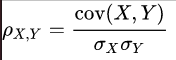
\includegraphics[scale=0.5]{imagens/R.png}}
\end{figure}

Mean Absolute Error\cite{abs}: It is the mean absolute difference between the measured values and “true” values.
\begin{figure}[H]
    \caption{Formula of Mean Absolute Error}\label{MAE}
    \centerline{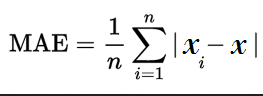
\includegraphics[scale=0.5]{imagens/MAE.png}}
\end{figure}
Root mean squared error\cite{rmse}: It represents the square root of the second sample moment of the differences between predicted values and observed values or the quadratic mean of these differences.
\begin{figure}[H]
    \caption{Formula of Root mean squared error}\label{RMSE}
    \centerline{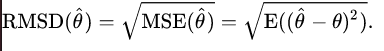
\includegraphics[scale=0.5]{imagens/RMSD.png}}
\end{figure}
Relative Absolute Error\cite{rae}: It is the ratio, comparing a mean error (residual) to errors produced by a trivial or naive model.
\begin{figure}[H]
    \caption{Formula of Relative Absolute Error}\label{RAE}
    \centerline{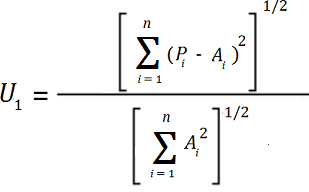
\includegraphics[scale=0.5]{imagens/RAE.png}}
\end{figure}
Root relative squared error\cite{rrse}: It is the measure of what the error would be if a simpler predictor had been used.
\begin{figure}[H]
    \caption{Formula of Root relative squared error}\label{RRSE}
    \centerline{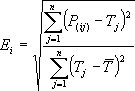
\includegraphics[scale=0.5]{imagens/RRSE.png}}
\end{figure}
\subsection{Parameter Configurations}
\paragraph{}
The 4 functions applied are have the following configurations:\break
LinearRegression -S 2 -R 1.0E-8 -num-decimal-places 4\hfill\break{}
GaussianProcesses -L 1.0 -N 0 -K "weka.classifiers.functions.supportVector.Puk -O 1.0 -S 1.0 -C 250007" -S 1\hfill\break{}
MultilayerPerceptron -L 0.3 -M 0.2 -N 500 -V 0 -S 0 -E 20 -H a\hfill\break{}
SMOreg -C 1.0 -N 0 -I "weka.classifiers.functions.supportVector.RegSMOImproved -T 0.001 -V -P 1.0E-12 -L 0.001 -W 1" -K "weka.classifiers.functions.supportVector.Puk -O 1.0 -S 1.0 -C 250007"\hfill\break{}

\subsection{Tables}

\begin{table}[H]
\caption{MeanArea predictions on Full Sample with Training set}\label{tab1}
\begin{tabular}{|l|l|l|l|l|l|}
\hline
RegFunction & Corre.\break Coef & Mean Abs Err & Root Mean Sqr Err & Rel Abs Err &Root Rel Sqr Err\\
\hline
LinearReg & 0.4344 & 7.7664 & 12.1085 & 87.4124 & 90.0712  \\
GaussProc & 0.996 & 4.568 & 6.9936 & 51.4142 & 52.0229 \\
MultiLayer & 0.9899 & 1.6445 & 2.0213 & 18.5097 & 15.0361 \\
SMOReg & 1 & 0.0704 & 0.0755 &  0.7927 & 0.5619 \\
\hline
\end{tabular}
\end{table}

\begin{figure}[H]
    \caption{Line Graph of True values vs Predictions, Mean Area, SMO, training set, full}\label{LGM}
    \centerline{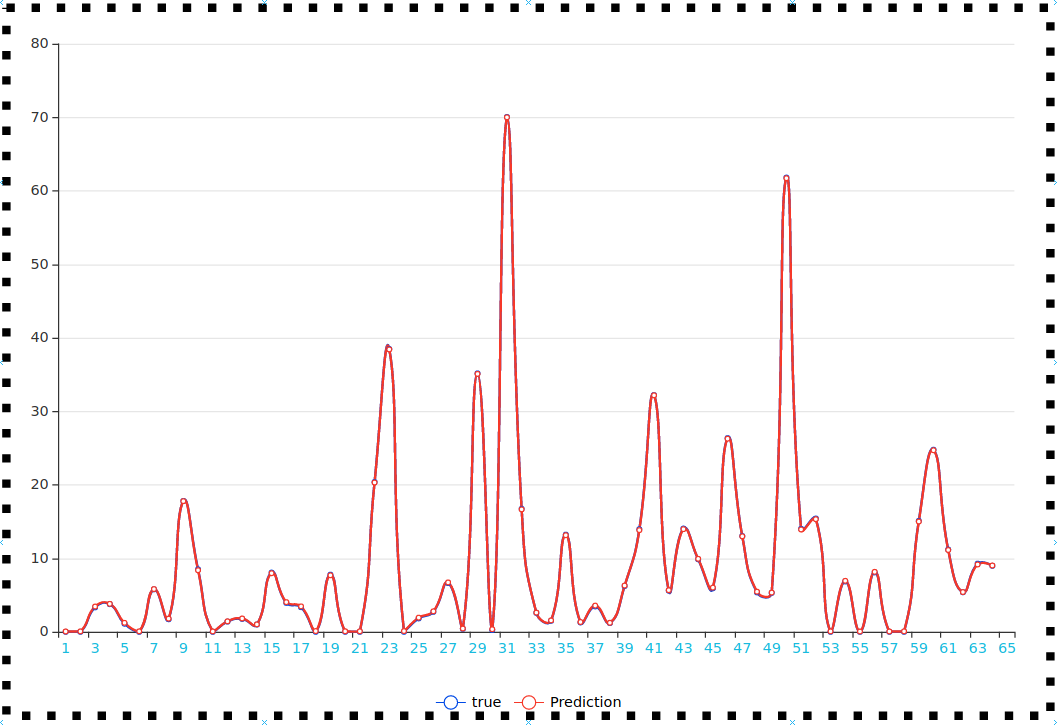
\includegraphics[width=1\columnwidth]{imagens/LineGraphMean.png}}
\end{figure}
\begin{figure}[H]
    \caption{Close up of Fig.10}\label{LGM2}
    \centerline{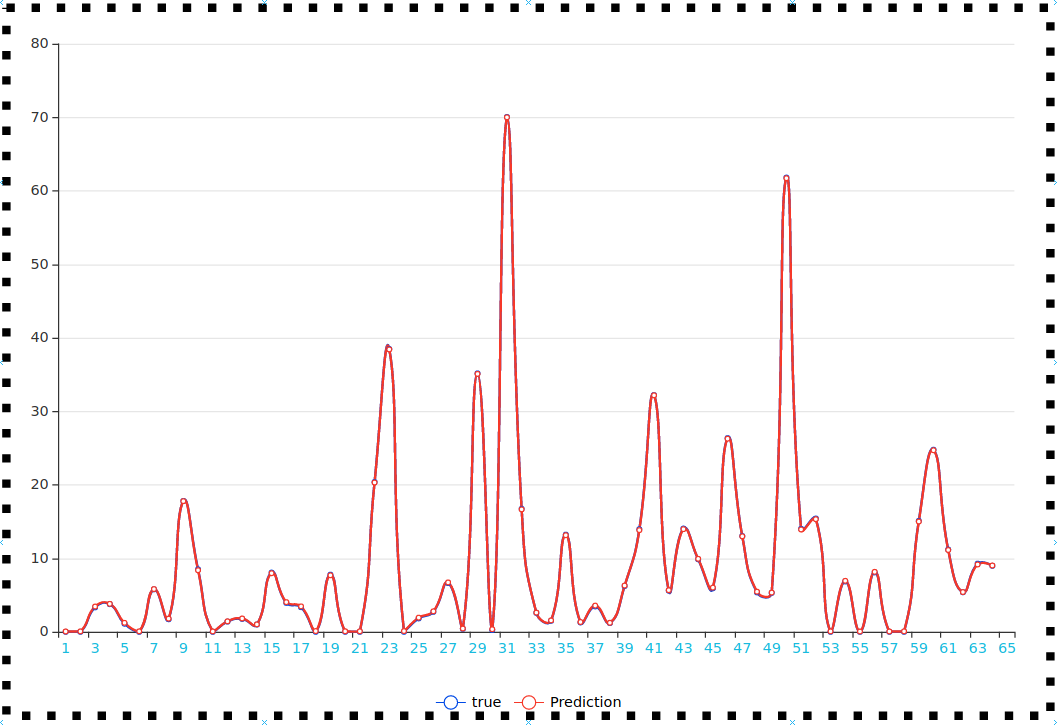
\includegraphics[width=1\columnwidth]{imagens/LineGraphMean.png}}
\end{figure}

\begin{table}[H]
\caption{NumberOfFires predictions on Full Sample with Training set}\label{tab2}
\begin{tabular}{|l|l|l|l|l|l|}
\hline
RegFunction & Corre.\break Coef & Mean Abs Err & Root Mean Sqr Err & Rel Abs Err &Root Rel Sqr Err\\
\hline
LinearReg & 0.936  & 2.2267 & 3.5335 & 28.3126  & 35.1909  \\
GaussProc & 0.9964 &3.4182& 4.452  & 43.4629 & 44.3386 \\
MultiLayer & 0.9966 & 0.9732 & 1.2264& 12.3742 & 12.3742\\
SMOReg & 1 &  0.0375 &0.0417 &   0.477 &  0.4154 \\
\hline
\end{tabular}
\end{table}
\begin{figure}[H]
    \caption{Line Graph of True values vs Predictions, Number Of Fires, SMO, training set}\label{LGN}
    \centerline{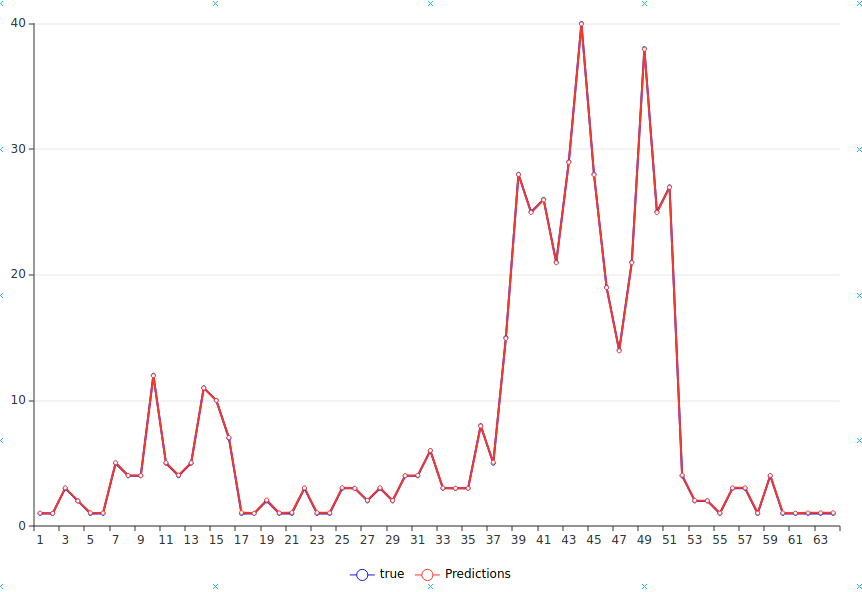
\includegraphics[width=1\columnwidth]{imagens/LineGraphNumber.png}}
\end{figure}

\begin{table}[H]
\caption{TotalAreaBurned predictions on Full Sample with Training set}\label{tab3}
\begin{tabular}{|l|l|l|l|l|l|}
\hline
RegFunction & Corre.\break Coef & Mean Abs Err & Root Mean Sqr Err & Rel Abs Err &Root Rel Sqr Err\\
\hline
LinearReg & 0.6684  & 83.4192 & 174.6733 &  63.6556 & 74.3841  \\
GaussProc &  0.9932 & 59.3553 & 114.8262 & 45.293 & 48.8984 \\
MultiLayer & 0.9992 & 14.1032 & 17.052 & 10.7619 & 7.2616\\
SMOReg & 1 &  1.6113 & 1.747 & 1.2296 & 0.744 \\
\hline
\end{tabular}
\end{table}

\begin{figure}[H]
    \caption{Line Graph of True values vs Predictions, Burned Area, SMO, training set}\label{LGMB}
    \centerline{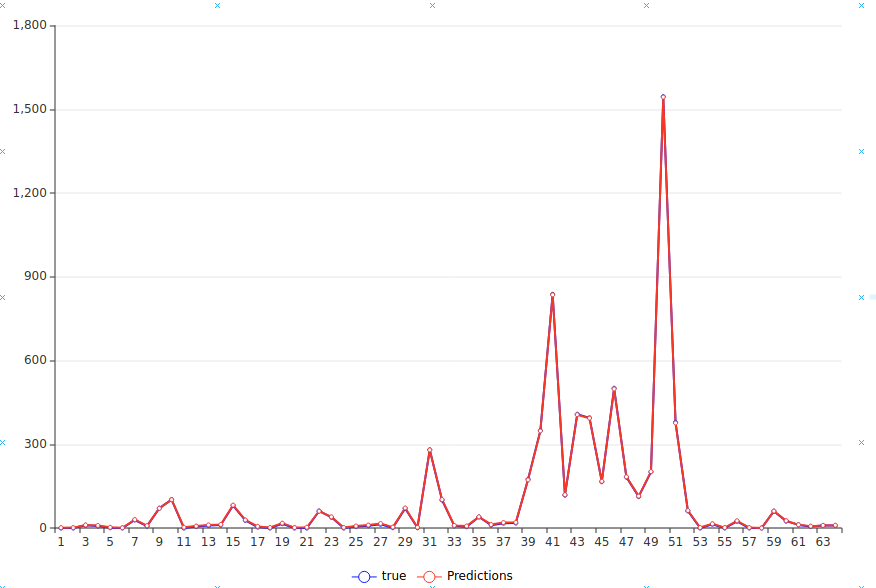
\includegraphics[width=1\columnwidth]{imagens/LinearGraphBurned.png}}
\end{figure}

\begin{table}[H]
\caption{MeanArea predictions on Full Sample with LOO Cross Validation}\label{tab4}
\begin{tabular}{|l|l|l|l|l|l|}
\hline
RegFunction & Corre.\break Coef & Mean Abs Err & Root Mean Sqr Err & Rel Abs Err &Root Rel Sqr Err\\
\hline
LinearReg & -0.0702 & 9.7319 & 15.1022 & 107.8229 & 110.585  \\
GaussProc & -0.1898 & 8.9577 & 13.7077 & 99.2453 & 100.3741 \\
MultiLayer & 0.001  & 19.9357 & 30.0635 & 220.8752 & 220.1387 \\
SMOReg & -0.1305 & 8.9465 & 13.8574 & 99.1212 & 101.4703 \\
\hline
\end{tabular}
\end{table}

\begin{table}[H]
\caption{NumberOfFires predictions on Full Sample with LOO Cross Validation}\label{tab5}
\begin{tabular}{|l|l|l|l|l|l|}
\hline
RegFunction & Corre.\break Coef & Mean Abs Err & Root Mean Sqr Err & Rel Abs Err &Root Rel Sqr Err\\
\hline
LinearReg & 0.8964 & 2.7361 & 4.4575 & 34.2454 & 43.6994  \\
GaussProc & 0.7882 & 6.7468 & 8.8109 & 84.4445 & 86.3779 \\
MultiLayer & 0.7979  & 4.3275 & 6.5258 & 54.164 & 63.9761 \\
SMOReg & 0.8162 & 5.8075 & 7.8432 & 72.6886 & 76.8916 \\
\hline
\end{tabular}
\end{table}

\begin{table}[H]
\caption{TotalAreaBurned  predictions on Full Sample with LOO Cross Validation}\label{tab6}
\begin{tabular}{|l|l|l|l|l|l|}
\hline
RegFunction & Corre.\break Coef & Mean Abs Err & Root Mean Sqr Err & Rel Abs Err &Root Rel Sqr Err\\
\hline
LinearReg & 0.4603 & 97.4797 & 214.8717 & 73.2227 & 90.0728  \\
GaussProc & 0.3785 & 117.0101 & 225.2621 & 87.8931 & 94.4284 \\
MultiLayer & 0.1772  & 182.3527 & 305.1051 & 136.9758 & 127.898 \\
SMOReg & 0.4166 & 109.4624 & 218.1673 & 82.2236 & 91.4542 \\
\hline
\end{tabular}
\end{table}

\begin{table}[H]
\caption{MeanArea predictions on Summer Sample with Training set}\label{tab7}
\begin{tabular}{|l|l|l|l|l|l|}
\hline
RegFunction & Corre.\break Coef & Mean Abs Err & Root Mean Sqr Err & Rel Abs Err &Root Rel Sqr Err\\
\hline
LinearReg & 0.3885 & 11.3618 & 16.0153 & 95.4163 & 92.1463  \\
GaussProc & 0.9986 & 6.2745 & 9.1554 & 52.6934 & 52.677 \\
MultiLayer & 1 & 0.1527 & 0.191 & 1.2824 & 1.0988 \\
SMOReg & 1 & 0.0734 & 0.0848 & 0.6162 & 0.4877 \\
\hline
\end{tabular}
\end{table}

\begin{table}[H]
\caption{NumberOfFires predictions on Summer Sample with Training set}\label{tab8}
\begin{tabular}{|l|l|l|l|l|l|}
\hline
RegFunction & Corre.\break Coef & Mean Abs Err & Root Mean Sqr Err & Rel Abs Err &Root Rel Sqr Err\\
\hline
LinearReg & 0.9235  & 3.4308 & 4.6205 & 31.5072  & 38.3659  \\
GaussProc & 0.9981 & 5.0719 & 5.6512 & 46.5789 & 46.925 \\
MultiLayer & 0.9999 & 0.1224 & 0.1538 & 1.1242 & 1.2768\\
SMOReg & 1 & 0.0381 & 0.042 & 0.3498 & 0.3485 \\
\hline
\end{tabular}
\end{table}

\begin{table}[H]
\caption{TotalAreaBurned predictions on Summer Sample with Training set}\label{tab9}
\begin{tabular}{|l|l|l|l|l|l|}
\hline
RegFunction & Corre.\break Coef & Mean Abs Err & Root Mean Sqr Err & Rel Abs Err &Root Rel Sqr Err\\
\hline
LinearReg & 0.6448  & 165.8187 & 249.2869 & 76.3631 & 76.439  \\
GaussProc & 0.9968 & 110.5328 & 165.5926 & 50.9028 & 50.7758\\
MultiLayer & 1 & 2.09 & 2.5715 & 0.9625 & 0.7885\\
SMOReg & 1 & 1.4186 & 1.5923 & 0.6533 & 0.4882\\
\hline
\end{tabular}
\end{table}

\begin{table}[H]
\caption{MeanArea predictions on Summer Sample with LOO Cross Validation}\label{tab10}
\begin{tabular}{|l|l|l|l|l|l|}
\hline
RegFunction & Corre.\break Coef & Mean Abs Err & Root Mean Sqr Err & Rel Abs Err &Root Rel Sqr Err\\
\hline
LinearReg & -0.3836 & 17.222 & 24.8046 & 139.2728 & 137.4311  \\
GaussProc & -0.7436 & 12.5731 & 18.3188 & 101.6775 & 101.496 \\
MultiLayer & -0.3187  & 30.0651 & 41.8752 & 243.134 & 232.0112 \\
SMOReg & -0.5781 & 12.7426 & 18.6339 & 103.0484 & 103.2418 \\
\hline
\end{tabular}
\end{table}

\begin{table}[H]
\caption{NumberOfFires predictions on Summer Sample with LOO Cross Validation}\label{tab11}
\begin{tabular}{|l|l|l|l|l|l|}
\hline
RegFunction & Corre.\break Coef & Mean Abs Err & Root Mean Sqr Err & Rel Abs Err &Root Rel Sqr Err\\
\hline
LinearReg & 0.7622 & 6.2662 & 7.8165 & 55.4151 & 62.5007  \\
GaussProc & 0.6047 & 10.2842 & 11.4497 & 90.9486 & 91.5515 \\
MultiLayer & 0.5565  & 10.3504 & 12.8984 & 91.5344 & 103.1348 \\
SMOReg & 0.7136 & 9.31 & 10.5489 & 82.3337 & 84.3485\\
\hline
\end{tabular}
\end{table}

\begin{table}[H]
\caption{TotalAreaBurned  predictions on Summer Sample with LOO Cross Validation}\label{tab12}
\begin{tabular}{|l|l|l|l|l|l|}
\hline
RegFunction & Corre.\break Coef & Mean Abs Err & Root Mean Sqr Err & Rel Abs Err &Root Rel Sqr Err\\
\hline
LinearReg & 0.2082 & 205.578 & 355.1582 & 91.1667 & 104.869  \\
GaussProc & -0.1844 & 221.6906 & 331.6897 & 98.3121 & 97.9394 \\
MultiLayer & 0.0634  & 470.9814 & 681.3341 & 208.864 & 201.1803 \\
SMOReg & 0.0636 & 214.0294 & 326.5549 & 94.9147 & 96.4232 \\
\hline
\end{tabular}
\end{table}



\subsection{Software}
\paragraph{}
These results were obtained using Weka\cite{weka}, an open source machine learning software containing several algorithms for data analysis, visualizations tools, pre-processing methods etc, it also features a free plugin store.
The histograms were made in www.meta-chart.com\cite{meta}, an online chart making website website and the line graphs in VisualParadigm\cite{vp}.


\subsection{Scripts}
\paragraph{}

The 2 aggregation scripts, named "aggregate.py" and "aggregateSummer.py" are located in the project folder.
I also wrote 2 scripts, named "getCount.py and getCountSummer.py", to count the number of fires for the linear scale of the histograms shown above, they are located in the project folder. 

\subsection{Attribute Selection}
\paragraph{}

Aside from deleting the X and Y attributes manually (through a script) and adding the 3 attributes I mentioned earlier, the only attribute selection applied lies in the "attributeSelectionMethod" parameter of the Linear Regression function in Weka, the options available were "No Attribute Selection", "Ms5 Method" and "Greedy Method". 
With the "Ms5 Method" the model sometimes predicts negative values when predicting some instances, which never makes sense because neither the number of fires nor the mean area burned nor the total area burned can be negative. Therefore these results were obtained using the "Greedy Method" which always predicts positive values.

\subsection{Time}
\paragraph{}
The aggregated dataset being so small meant that, performance wise, most of the classification algorithms applied finish very fast. Only Multilayer Perceptron with leave one out cross validation and with the full sample took 35s


\section{Conclusions}
\paragraph{}
From the 3 attributes, the one that every algorithm can predict reasonably well seems to be the number of fires.


I found that one big limitation of every model that Weka came up with was missing data, the fact is that we have no information on the pairs of DOW/Month when there weren't any fires, meaning that the aggregated dataset is missing 20 instances that could've been beneficial to the model. I thought about inserting these instances myself to fill in the blanks but realized I would need information on the temperature, rain, wind etc of Montesinho natural park in 2003 which I couldn't find. 

So in regards to future work with this dataset or with this type of problem, I would try to obtain a more complete set of data to fill in the 20 instance empty space in the aggregated data set. These 20 extra instances would have a mean area burned, number of fires and total burned area of 0 but their meteorological information (the average temperature, rain, wind in that DOW/Month) might give valuable information to the model.



\printbibliography
\end{document}